\documentclass{beamer}
\usepackage[utf8]{inputenc}

\usetheme{Madrid}
\usecolortheme{default}
\usepackage{amsmath,amssymb,amsfonts,amsthm}
\usepackage{txfonts}
\usepackage{tkz-euclide}
\usepackage{listings}
\usepackage{adjustbox}
\usepackage{array}
\usepackage{tabularx}
\usepackage{gvv}
\usepackage{lmodern}
\usepackage{circuitikz}
\usepackage{tikz}
\usepackage{graphicx}

\setbeamertemplate{page number in head/foot}[totalframenumber]

\usepackage{tcolorbox}
\tcbuselibrary{minted,breakable,xparse,skins}



\definecolor{bg}{gray}{0.95}
\DeclareTCBListing{mintedbox}{O{}m!O{}}{%
  breakable=true,
  listing engine=minted,
  listing only,
  minted language=#2,
  minted style=default,
  minted options={%
    linenos,
    gobble=0,
    breaklines=true,
    breakafter=,,
    fontsize=\small,
    numbersep=8pt,
    #1},
  boxsep=0pt,
  left skip=0pt,
  right skip=0pt,
  left=25pt,
  right=0pt,
  top=3pt,
  bottom=3pt,
  arc=5pt,
  leftrule=0pt,
  rightrule=0pt,
  bottomrule=2pt,
  toprule=2pt,
  colback=bg,
  colframe=orange!70,
  enhanced,
  overlay={%
    \begin{tcbclipinterior}
    \fill[orange!20!white] (frame.south west) rectangle ([xshift=20pt]frame.north west);
    \end{tcbclipinterior}},
  #3,
}
\lstset{
    language=C,
    basicstyle=\ttfamily\small,
    keywordstyle=\color{blue},
    stringstyle=\color{orange},
    commentstyle=\color{green!60!black},
    numbers=left,
    numberstyle=\tiny\color{gray},
    breaklines=true,
    showstringspaces=false,
}
%------------------------------------------------------------
%This block of code defines the information to appear in the
%Title page
\title %optional
{1.9.21}
\date{August 26,2025}


\author 
{Kartik Lahoti - EE25BTECH11032}



\begin{document}


\frame{\titlepage}
\begin{frame}{Question}
Given vertices of a parallelogram $\vec{A} \brak{-2,1} , \vec{B} \brak{a,0} , \vec{C} \brak{4,b}, \text{ and } \vec{D} \brak{1,2}$. Find the values of $a \text{ and } b $. Hence, find the lengths of its sides.
\end{frame}



\begin{frame}{Theoretical Solution}
Given,

A parallelogram $ABCD$ with , 
\begin{align}
    \vec{A} = \myvec{-2\\1} , \vec{B} = \myvec{a\\0} , \vec{C} = \myvec{4\\b} , \vec{D} = \myvec{1\\2}     
\end{align}

\end{frame}

\begin{frame}{Theory}

In a Parallelogram $PQRS$ the opposite side are parallel and equal , i.e. $PQ \parallel RS $ and $PQ = RS $ and similarly  $QR \parallel  PS $ and $ QR = PS $

$\therefore$ \text{Here we can say, } \begin{align}\vec{AB} = \vec{DC}\end{align}
\end{frame}
\begin{frame}{Theoretical Solution}

Calculating $\vec{AB}$ , 

\begin{align}
    \vec{AB} = \vec{B} - \vec{A}
\end{align}

\begin{align}
    \vec{AB} &= \myvec{a\\0} - \myvec{-2\\1} = \myvec{a+2\\-1}
\end{align}

Similarly, 
\begin{align}
    \vec{DC} &= \myvec{3\\b-2}
\end{align}

\end{frame}

\begin{frame}{Theoretical Solution}
From Eqn (2) we get : 
\begin{align}
    \myvec{a+2\\-1} = \myvec{3\\b-2} \\
\end{align}
\begin{align}
    \implies a = 1 \text{ and }  b = 1
 \end{align}

$\therefore a = 1$ and $ b = 1 $ 

\end{frame}

\begin{frame}{Theoretical Solution}
    Calculating the side lengths , 

\begin{align}
    \because \vec{A} - \vec{B} = \myvec{-3\\1} , \\
    (\vec{A} - \vec{B})^\top (\vec{A} - \vec{B}) &=  10
\end{align}
Thus, the desired length $\vec{AB}$ is 
\begin{align}
		d_1=\norm{\vec{A}-\vec{B}} =\sqrt{10}
\end{align}
\end{frame}

\begin{frame}{Theoretical Solution}

Similarly, 
\begin{align}
    \because \vec{B} - \vec{C} = \myvec{-3\\-1} , \\
    (\vec{B} - \vec{C})^\top (\vec{B} - \vec{C}) &=  10
\end{align}
Thus, the desired length $\vec{BC}$ is 
\begin{align}
		d_2=\norm{\vec{B}-\vec{C}} =\sqrt{10}
\end{align}

\textbf{Hence: } The length of the sides of the parallelogram is $ \sqrt{10} $
    
\end{frame}

\begin{frame}[fragile]
    \frametitle{C Code (1) - Function to Magnitude of Vector AB }

    \begin{lstlisting}

#include <math.h>
double length(double *A , double *B , int m )
{
    double sum = 0.0; 
    for ( int i = 0 ; i < m ; i++ )
    {
        sum += pow(A[i]-B[i] , 2 );
    }
    return sqrt(sum) ; 
}

    \end{lstlisting}
\end{frame}



\begin{frame}[fragile]
    \frametitle{C Code (2) - Function to Generate Points on Line}
    \begin{lstlisting}

void linegen(double *X, double *Y , double *A , double *B , int n , int m )
{
    double temp[m] ; 
    for (int i = 0 ; i < m ; i++)
    {
        temp [ i ] = (B[i]- A[i]) /(double) n ; 
    }
    for (int i = 0 ; i <= n ; i++ )
    {
        X[i] = A[0] + temp[0] * i ; 
        Y[i] = A[1] + temp[1] * i ;
    }
}

\end{lstlisting}
\end{frame}

\begin{frame}[fragile]
    \frametitle{Python Code - Using Shared Object}
    \begin{lstlisting}
import ctypes
import numpy as np
import matplotlib.pyplot as plt
def length_func (P: np.ndarray , Q: np.ndarray, m ) -> float:
    handc1 = ctypes.CDLL("./length.so")

    handc1.length.argtypes = [
        ctypes.POINTER(ctypes.c_double),
        ctypes.POINTER(ctypes.c_double),
        ctypes.c_int    ]
    handc1.length.restype = ctypes.c_double

    len = handc1.length (
        P.ctypes.data_as(ctypes.POINTER(ctypes.c_double)),
        Q.ctypes.data_as(ctypes.POINTER(ctypes.c_double)),
        m   )
    return len



\end{lstlisting}
\end{frame}

\begin{frame}[fragile]
    \frametitle{Python Code - Using Shared Object}
    \begin{lstlisting}
    
A = np.array([[-2],[1]], dtype=np.float64)
B = np.array([[1],[0]], dtype=np.float64)
C = np.array([[4],[1]], dtype=np.float64)
D = np.array([[1],[2]], dtype=np.float64)

d1 = length_func(A,B,2)
d2 = length_func(B,C,2)

if d1 == d2 :
    print("Length of Sides =",d1)
else:
    print("Length of Side AB and CD = ",d1)
    print("Length of Side BC and AD = ",d2)

\end{lstlisting}
\end{frame}

\begin{frame}[fragile]
    \frametitle{Python Code - Using Shared Object}
    \begin{lstlisting}

def line_cre(P: np.ndarray , Q: np.ndarray, str):
    handc2 = ctypes.CDLL("./line_gen.so")

    handc2.linegen.argtypes = [
        ctypes.POINTER(ctypes.c_double),
        ctypes.POINTER(ctypes.c_double),
        ctypes.POINTER(ctypes.c_double),
        ctypes.POINTER(ctypes.c_double),
        ctypes.c_int , ctypes.c_int
    ]

    handc2.linegen.restype = None
    


\end{lstlisting}
\end{frame}
\begin{frame}[fragile]
    \frametitle{Python Code - Using Shared Object}
    \begin{lstlisting}
n = 200
    X_l = np.zeros(n,dtype=np.float64)
    Y_l = np.zeros(n,dtype=np.float64)

    handc2.linegen (
        X_l.ctypes.data_as(ctypes.POINTER(ctypes.c_double)),
        Y_l.ctypes.data_as(ctypes.POINTER(ctypes.c_double)),
        P.ctypes.data_as(ctypes.POINTER(ctypes.c_double)),
        Q.ctypes.data_as(ctypes.POINTER(ctypes.c_double)),
        n,2
    )
    plt.plot([X_l[0],X_l[-1]],[Y_l[0],Y_l[-1]],str)

    \end{lstlisting}
\end{frame}

\begin{frame}[fragile]
    \frametitle{Python Code - Using Shared Object}
    \begin{lstlisting}

plt.figure()

line_cre(A,B,"g-")
line_cre(B,C,"r-")
line_cre(C,D,"b-")
line_cre(D,A,"y-")

coords = np.block([[A,B,C,D]])
plt.scatter(coords[0,:],coords[1,:])
vert_labels = ['A','B','C','D']
#for i , txt in enumerate(vert_labels):
 #   plt.annotate(txt,(coords[0,i],coords[1,i]),textcoords="offset points", xytext=(0,10),ha='center')



\end{lstlisting}
\end{frame}

\begin{frame}[fragile]
    \frametitle{Python Code - Using Shared Object}
    \begin{lstlisting}
for i, txt in enumerate(vert_labels):
    plt.annotate(f'{txt}\n({coords[0,i]:.0f}, {coords[1,i]:.0f})',
                 (coords[0,i], coords[1,i]),
                 textcoords="offset points",
                 xytext=(20,0),
                 ha='center')


plt.xlabel('$x$')
plt.ylabel('$y$')
#plt.legend(loc='best')
plt.grid()
\end{lstlisting}
\end{frame}

\begin{frame}[fragile]
    \frametitle{Python Code - Using Shared Object}
    \begin{lstlisting}

plt.title("Fig:1.9.21")
plt.axis('equal')

plt.savefig("../figs/p_gram1.png")
plt.show()

#plt.savefig('figs/triangle/ang-bisect.pdf')
#subprocess.run(shlex.split("termux-open figs/triangle/ang-bisect.pdf"))

\end{lstlisting}
\end{frame}




\begin{frame}[fragile]
    \frametitle{Python Code}
    \begin{lstlisting}
import math
import sys 
sys.path.insert(0, '/home/kartik-lahoti/matgeo/codes/CoordGeo')
import numpy as np
import numpy.linalg as LA
import matplotlib.pyplot as plt
import matplotlib.image as mpimg

from line.funcs import *
#from triangle.funcs import *
#from conics.funcs import circ_gen


#if using termux
#import subprocess
#import shlex
\end{lstlisting}
\end{frame}

\begin{frame}[fragile]
    \frametitle{Python Code }
    \begin{lstlisting}

def length(P,Q) :
    return LA.norm(P-Q)

A = np.array([-2,1]).reshape(-1,1)
B = np.array([1,0]).reshape(-1,1)
C = np.array([4,1]).reshape(-1,1)
D = np.array([1,2]).reshape(-1,1)

d1 = length(A,B)
d2 = length(B,C)
if d1 != d2 :
    print("Length of AB and CD = ",d1)
    print("Length of BC and AD = ",d2)
else :
    print("Length of all sides = ",d1)


\end{lstlisting}
\end{frame}

\begin{frame}[fragile]
    \frametitle{Python Code }
    \begin{lstlisting}

def plot_it(P,Q,str):
    x_l = line_gen_num(P,Q,20)
    plt.plot(x_l[0,:],x_l[1,:] , str )

plt.figure()

plot_it(A,B,"g-")
plot_it(B,C,"r-")
plot_it(C,D,"b-")
plot_it(D,A,"y-")
\end{lstlisting}
\end{frame}

\begin{frame}[fragile]
    \frametitle{Python Code }
    \begin{lstlisting}

coords = np.block([[A,B,C,D]])
plt.scatter(coords[0,:],coords[1,:])
vert_labels = ['A','B','C','D']
#for i , txt in enumerate(vert_labels):
 #   plt.annotate(txt,(coords[0,i],coords[1,i]),textcoords="offset points", xytext=(0,10),ha='center')
for i, txt in enumerate(vert_labels):
    plt.annotate(f'{txt}\n({coords[0,i]:.0f}, {coords[1,i]:.0f})',
                 (coords[0,i], coords[1,i]),
                 textcoords="offset points",
                 xytext=(20,0),
                 ha='center')


    \end{lstlisting}
\end{frame}
\begin{frame}[fragile]
    \frametitle{Python Code }
    \begin{lstlisting}

    
plt.xlabel('$x$')
plt.ylabel('$y$')
#plt.legend(loc='best')
plt.grid()

plt.title("Fig:1.9.21")
plt.axis('equal')

plt.savefig("../figs/p_gram2.png")
plt.show()

#plt.savefig('figs/triangle/ang-bisect.pdf')
#subprocess.run(shlex.split("termux-open figs/triangle/ang-bisect.pdf"))

    \end{lstlisting}
\end{frame}


\begin{frame}{Plot}
    \centering
    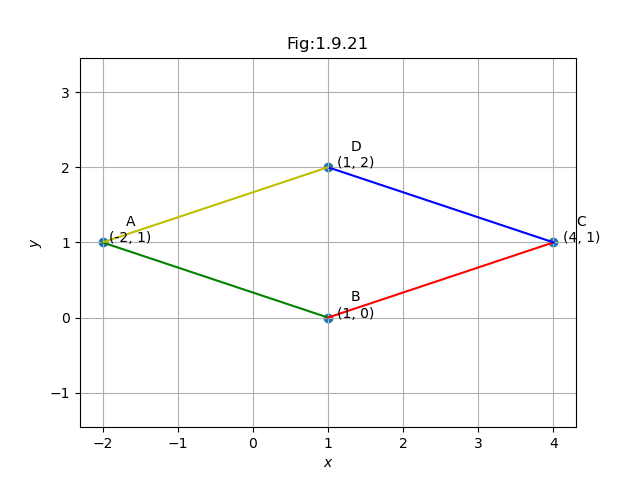
\includegraphics[width=\columnwidth, height=0.8\textheight, keepaspectratio]{figs/p_gram1.png}   
\end{frame}


\end{document}
